\chapter{Related Work - Stack of Tasks}
\label{chapter:soth}

The Stack-of-Tasks (SoT) is an efficient framework for hierarchical quadratic programming (QP) \cite{kanoun:itro:11}. It implements a General Inverse Kinematics (GIK), which was firstly presented in \cite{nakamura}. A task denotes an abstract desired goal value, which can be achieved by controlling an ordinary differential equation \cite{ROB:2555180}. Tasks can be, among others, a desired pose of a manipulator, a gaze task describing a point in a 2-dimensional plane or a range of allowed joint values. Whole body motion control implies a high number of DoF and with it a lot of redundancy. Thus it becomes obvious that multiple instances of those tasks can be regulated simultaneously \cite{Liegeois1977}. A widely common approach is to install a hierarchy of tasks, solving them recursively in respect of the precedent nullspace \cite{siciliano1991general}.  \\
\\
Generally, the SoT provides two main functionalities. Firstly, it incorporates a QP solver in a hierarchy preserving manner \cite{mansard-tro-09}. Hereby, a novel and highly computationally efficient matrix decomposition was introduced, which yields a remarkable improvement in terms of computation speed \cite{escande-ijrr-sub12}. \cite{escande-icra-10} refers to this specific development as Hierarchical Complete Orthogonal Decomposition (HCOD), which is adopted throughout this work when the emphasis is attached to the solver itself rather than the overall framework.\\
\\
Secondly, the SoT describes a software framework, which implements an intelligent way of establishing a dynamic hierarchy by activating and deactivating task constraints on runtime. In the remainder of this chapter, the focus lies on the theoretical aspect of numerically solving the hierarchy of tasks. Complementary, the implementation of the software framework takes place in the second part of this work in chapter \ref{chapter:implenv}.

\section{Prerequisites}
The SoT is the base line of this work. In order to ease the understanding of the concepts presented in the following, a few requisites are recalled. The inverse kinematic solver mainly works with a least-square pseudo inverse approach, which can be formulated as a constrained quadratic programming problem. Finally, the SoT implements an inverse kinematics control scheme to run in real time on the robot.
\subsection{Least Square}
Least Squares is a way to optimize problems to its best. It applies always to overdetermined problems, where there exists no unique solution. This is the case, when there are more linearly independent equations than unknowns. 
\begin{equation}\label{eqn:leastsquare}
Ax = b \quad \text{with } A \in \mathbb{R}^{m \times n}, m < n
\end{equation}
Since $A$ is strictly skinny matrix, there is no direct inverse in order to analytically solve this equation system. However, we can optimize this system to its best, meaning we minimize the resulting error, when we take all equations into consideration. Equation \ref{eqn:leastsquare} thus turns into
\begin{equation}\label{leastsquareerror}
r = Ax -b
\end{equation}
The optimization is formulated as follows:
\begin{equation}
x^* =  \underset{x}{\text{arg min}} \left\| Ax - b \right \|
\end{equation}
The solution can be found by minimizing the squared residual. Minimizing means computing a solution for the first derivative set to zero.
\begin{eqnarray}
\left\| r \right\|^2 &=& xA^TAx - 2b^TAx + b^Tb  \label{eqn:leastsquarevebose}\\
\nabla_x \left\| r \right\|^2 &=& 2 A^TAx - 2A^Tb = 0
\end{eqnarray}
This further yields to the solution of the normal equation
\begin{eqnarray}
A^TAx &=& A^Tb \\
x &=& A^T(A^TA)^{-1} b \\ \label{eqn:pseudoinverse}
x &=& A^+b
\end{eqnarray}
where equation \ref{eqn:pseudoinverse} describes the famous Moore-Penrose pseudo inverse.

\subsection{Quadratic Programming}
Quadratic Programming handles optimization problems with linear equality or inequality constraints. Hence the name, the primal objective function to optimize is a quadratic function. The general problem statement can be formulated as follows:
\begin{eqnarray}\label{eqn:qp}
\frac{1}{2}x^TQx + c^Tx + r_o \\
\text{subject to } Dx = e \quad \in \mathcal{E} \\
\text{subject to } Dx \leq e \quad\in \mathcal{I} 
\end{eqnarray}
Since the objective function describe a quadratic function, a least square formulation can be easily transformed into a QP. 
From the equation in \ref{eqn:leastsquarevebose}, it can be easily seen that this equation has the same shape as equation \ref{eqn:qp}.

We can solve general QP problems by applying Lagrange multiplier for each constraints. We formulate the Lagrangian equation by multiplying each constraint and optimize for $x$ and $\lambda$.
\begin{equation}\label{eqn:lagrangian}
\mathcal{L}(x,\lambda) = \frac{1}{2}x^TQx + c^Tx + r_o + \lambda^T (Dx-e)
\end{equation}
The Karush-Kuhn-Tucker conditions \cite{kuhn50nonlinear} for this are given as follows
\begin{eqnarray}
\nabla \mathcal{L}(x, \lambda) &=& 0 \\
d_i^Tx &=& e_i \quad \in \mathcal{E} \\
d_i^Tx &\geq & e_i \quad \in \mathcal{I} \\
\lambda &\geq & 0 \quad \in \mathcal{I} \\ \label{eqn:kktineq1} 
\lambda (d_i^Tx-e_i) &=& 0 \quad \in \mathcal{I} \label{eqn:kktineq2} 
\end{eqnarray}
When we look closer at the last two conditions \ref{eqn:kktineq1} and \ref{eqn:kktineq2}, we can see that all active inequality constraints have to be satisfied. Condition \ref{eqn:kktineq1} emphasizes that only constraints are valid and thus optimized, where their according $\lambda$ is positive. Conditions with positive Lagrange multipliers are not considered to contribute to an optimal solution. Moreover, inequalities are called satisfied, when the optimal solution lies directly on the border. Thus, an inequality turns into an equality constraint (condition \ref{eqn:kktineq2}) and can be solved in a least square sense. 

Considering those two conditions, we always have to find the optimal set of inequality constraints, which are active and thus can be solved in a equality like behavior. Prominent approaches are Simplex algorithms \cite{murty1983linear} and Active Set Search\cite{GVK502988711} methods. The latter will be explained in more detail in the remainder of this chapter. 


\subsection{Inverse Kinematics Control Scheme}\label{subsec:ik}
GIK can be solved with a geometrical approach\cite{c1983geometric} just to a certain extend \cite{citeulike:1090825}. When the number of actuated joints increases, in particular in redundant manipulators, an numerical approach for solving the inverse kinematics problem is widely chosen \cite{springer}. The differential equation for the inverse kinematics describes a linear mapping between cartesian space and operational space
\begin{equation}
\vec{\dot{x}} = \vec{J}\vec{\dot{q}}
\end{equation}
where $\vec{\dot{x}}$ denotes a velocity in cartesian space, whereas $\vec{\dot{q}}$ defines the robot control input vector. The Jacobian matrix $\vec{J}$ describes the linear mapping function between the two spaces. From the above formulation, we can see the similarity to the least squares equations. Thus, since a redundant manipulator describes an overdetermined system, it makes sense to solve this optimization problem with a pseudo-inverse approach.
\begin{equation} \label{eqn:inverseIK}
\vec{\dot{q}} = \vec{J}^+\vec{\dot{x}}
\end{equation}
Redundant manipulator implies a set of possible solutions, since the system is overdetermined and thus comprises unused DoF. Those unused DoF can be used to cascade secondary objectives without violating the first constraint \cite{12020}. In order to achieve this, we can freely multiply any arbitrary vector $\vec{q_1}$ with the according projection $\vec{P_0}$ into the nullspace of the primal objective function. Therefore, we extend equation \ref{eqn:inverseIK} to
\begin{equation} \label{eqn:inverseIKnullspace}
\vec{\dot{q}} = \vec{J}_0^+\vec{\dot{x}_0} + \vec{P}_0\vec{\dot{q}}_1 
\end{equation}
where $\vec{P}$ is defined as $\vec{I} - \vec{J}^+\vec{J}$.

This formulation can be included into a real time constrained control scheme. The partial velocities, solved with the above method, are integrated over time and the resulting joint positions $\vec{q}$ are set on the respective motors. The control scheme can be formulated as follows:
\begin{equation}
\vec{q}(t_{k+1}) = \vec{q}(t_{k}) + [ \vec{J}(t_{k+1})^+\vec{\dot{x}}(t_{k+1}) + \vec{P}\vec{\dot{q}}(t_{k+1}) ] \Delta t
\end{equation}
However, since the control scheme is mainly driven by a forward control design, it makes sense to put this control scheme in dependency of a desired cartesian position $\vec{x_d}$ and regulate the resulting error between actual solution and desired position.
We formulate the error equation by incorporating the desired values
\begin{equation}\label{eqn:ikfirstorder}
\vec{\dot{e}} =  \vec{\dot{x}}_d - \vec{\dot{x}} =  \vec{\dot{x}}_d - \vec{J}\vec{\dot{q}}
\end{equation}
When we look in particular at equation \ref{eqn:ikfirstorder}, we can see a first-order differential equation. The solution as written in equation \ref{eqn:inverseIK} thus becomes
\begin{eqnarray}
\vec{\dot{q}} &=& \vec{J}^+\vec{\dot{e}} \\
			   &=& \vec{J}^+(\vec{\dot{x}}_d - \vec{\dot{x}})
\end{eqnarray}
Additionally, to complement the control law, a proportional constant $K$ is introduced as a gain parameter to optimize the convergence speed. The overall controller can be illustrated in the following diagram (figure \ref{fig:ikcontrolloop}).
\begin{figure}[h!]
  \centering
    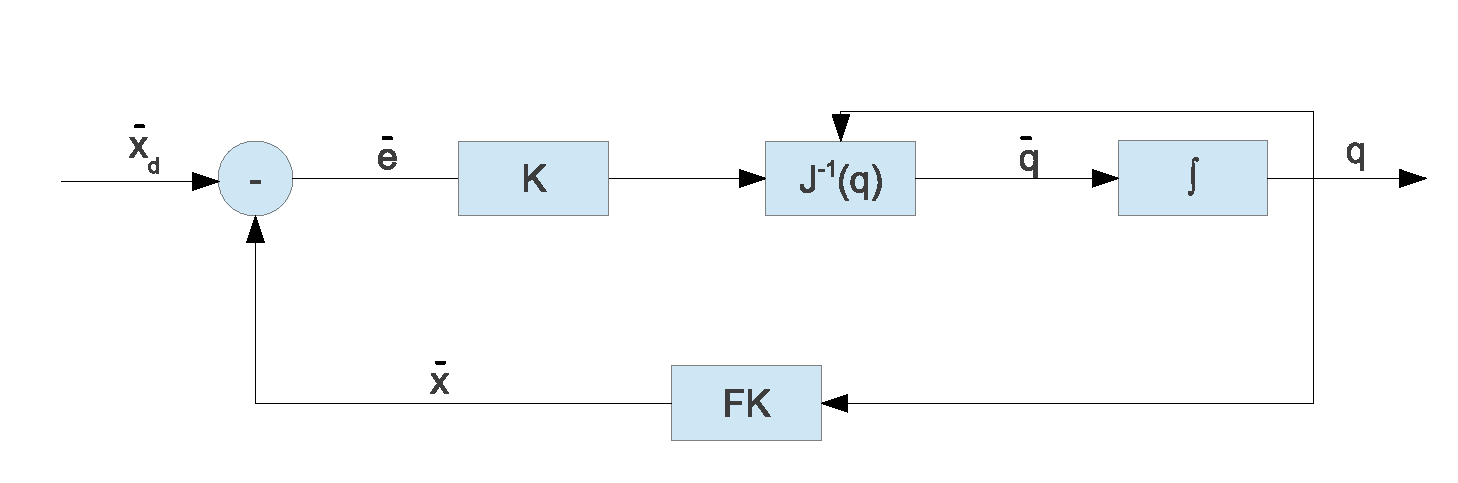
\includegraphics[width=0.8\textwidth]{../figures/ikcontrolloop.eps}
    \caption{Illustration of the Inverse Kinematics control scheme. The error is computed via the desired position $x_d$ and the current velocity provided by the Forward Kinematics $FK$.}
    \label{fig:ikcontrolloop}
\end{figure}
\section{Hierarchical Inverse Kinematics}
Current state of the art humanoid robots possess around 30-40 DoF. This allows an execution of multiple tasks in parallel. We start our examination by firstly looking at one task. When we want to control any actuated end-effector, we consume 6 DoF in $SE(3)$ Lie group \cite{LIE} for a full pose positioning. A simple manipulating task can be formulated based on a task space value $\vec{\dot{e}}$, with an unknown joint vector $\vec{\dot{q}}$ and the translating Jacobian $\vec{J}= \frac{\partial e}{\partial q}$.
\begin{equation}\label{eqn:ikcontrol}
\vec{\dot{e}} = \vec{J}\vec{\dot{q}}
\end{equation}
where $\vec{\dot{q}}$ describe the solution vector in joint velocity space, which will serve as the input of the robot.
The GIK formulation in equation \ref{eqn:ikcontrol} can be solved in a least square approach, solving the following QP to its best:
\begin{equation}\label{eqn:ikleastsquare}
\vec{\dot{q}^*} =  \underset{\dot{q}}{\text{arg min}} \left\| \vec{J}\vec{\dot{q}} - \vec{\dot{e}^*} \right \|
\end{equation}
The above QP formulation is broadly used for inverse kinematics \cite{Whitney72a}\cite{Chiaverini94reviewof} or inverse dynamics \cite{khatib-1987a}. For the remainder of this chapter, we consider a general least square approach and rename equation \ref{eqn:ikleastsquare} into
\begin{equation}\label{eqn:ikleastsquaresol}
x^* =  \underset{x}{\text{arg min}} \left\| Ax - b \right \|
\end{equation}
The solution for this optimization problem can be found by utilizing the pseudo-inverse approach \cite{journals/jirs/Siciliano90}, which yields to
\begin{equation}\label{eqn:ikleastsquaresolinv}
x^* = A^+ b \quad \text{with }A^+ = A^T(AA^T)^{-1}
\end{equation}
where $A^+$ denotes the Moore-Penrose pseudo-inverse \cite{ben2003generalized}. Considering a set of constraints, \ref{eqn:ikleastsquaresol} can be enhanced by a nullspace projection \cite{Liegeois1977} to obtain a generic solution.
\begin{equation}\label{eqn:ikleastsquarenullspace}
x^* = A^+ b  + Px_p
\end{equation}
where $P$ denotes the projection of an arbitrary vector $x_p$ into the nullspace of $A_1$. 
However, since we have a high number of redundant joints, we can execute multiple tasks in parallel. Thus, a task can be positioning an arm end-effector, keeping the vision system orientated towards a fixed point in 3-dimensional space or use both legs for walking. On the other hand, multiple tasks might not be feasible, since they either share common parts of the kinematic chain (e.g. torso links between the left and right arm) or interfere with each other. The idea is to implement a hierarchy of tasks, where the highest priority task will be solved to its best in a least square approach, whereas lower prioritized tasks are solved inside the of each respective precedent nullspace.

Equation \ref{eqn:ikleastsquarenullspace} allows us to include a secondary constraint into the QP, which does not violate the primal objective function. Considering now two tasks, we can setup a simple hierarchy based on that nullspace projection. Let $A_1,b_1$ be the primal objective and $A_2,b_2$ a secondary task, we can formulate the following hierarchical QP, substituting equation \ref{eqn:ikleastsquarenullspace} into \ref{eqn:ikleastsquaresol}:
\begin{eqnarray}
x_2^* =  \underset{x_2}{\text{arg min}} & \left\| A_2x_2 - b_2 \right \| \notag \\
& \left\| A_2(A_1^+b_1+P_1x_2) - b_2 \right \| \notag \\
& \left\| A_2P_1x_2 - (b_2 - A_2A_1^+b_1) \right \|
\end{eqnarray}
The generic solution for this QP, can be equally as in equation \ref{eqn:ikleastsquarenullspace} found with the pseudo-inverse:
\begin{equation}\label{eqn:ikleastsquarenullspaceexample}
x_2^* = (A_2P_1)^+ (b_2 - A_2A_1^+b_1)  + P_2x_3
\end{equation}
This implies that a solution for lower stacked tasks can only be found if there exists a nullspace of a precedent task. If the above task consumes all DoF, lower placed tasks can not be considered any further.

The above equation \ref{eqn:ikleastsquarenullspaceexample} is recursively formulated in \cite{siciliano1991general} for $n$ hierarchically stacked tasks.
\begin{equation}\label{eqn:ikleastsquarerecursive}
x^*_n = \sum_{k=1}^n (A_kP_{k-1})^+ (b_k - A_{k}A_{k-1}^+b_{k-1}) + P_nx_{n+1}
\end{equation}

\section{Inequality Constraints}
The above presented hierarchy describes a equality constrained Quadratic Program (eQP). This enables a simultaneous execution of multiple tasks with equality constraints, such as positioning tasks. However, in order to implement safety mechanism, no hard constraints but solution spaces are necessary, which immediately demand for inequality constraints. Safety mechanisms can be such as an active elbow-field, keeping the elbow above a certain threshold, balancing the center of mass (CoM) inside a polygon or avoiding collision with obstacles, as it is the topic of this work.

We can formulate an inequality Quadratic Program (iQP) in a classical manner:
\begin{eqnarray}
x^* =  \underset{x}{\text{arg min}} \left\| Ax - b \right \| \\
\text{subject to } Cx < d
\end{eqnarray} 
\newpage
These kind of iQP are often formulated by introducing a slack variable $w$, which indicates the level of violation \cite{kanoun:inria-00390581}. 
\begin{eqnarray} \label{eqn:ikineq}
x^*, w^* =  \underset{x,w}{\text{arg min}} \left\| w \right \| \\
\text{subject to } Cx < d + w
\end{eqnarray} 

Let us assume that $Cx <d$ fulfills all the KKT \cite{kuhn50nonlinear} conditions. We can then denote this an optimal solution set and easily solve this iQP as if it were an eQP. This means, that in an optimal set of inequalities, the solution satisfies all active constraints \cite{escande-icra-10}.

The main idea of solving such an iQP is finding the set of constraints, which form the optimal set. Those algorithms are mainly referred as Active Set Search \cite{GVK502988711} and often used to solve inequality constraint QPs. The algorithms starts with an initial guess $\vec{x}_0$ and working set $\vec{W}$ filled with activated constraints. The first step is to solve the iQP like an eQP and find the KKT optimal conditions $\vec{x}_{t=1}, \vec{\lambda}_{t=1}$. When one or many Lagrange multiplier are negative, the currently active set is not optimal, which means there are unnecessary constraints. The negative constraint $\lambda_k$ is dismissed and the algorithm starts over again with $\vec{x}_0$ and $\{ \vec{W} \setminus \lambda_k \}$ in order to solve $\vec{x}_{t=2}, \vec{\lambda}_{t=2}$. 

Once a solution is found, where $\vec{\lambda}$ is strictly positive, we perform a search step. This is by best practice performed in the direction of $\vec{v} = \vec{x}_1-\vec{x}_2$. 
\begin{equation*}
\vec{x^*_1} = \vec{x_1}+ p\vec{v} \quad \text{with } p \in [0;1]
\end{equation*}
We have to prove the new step for feasibility. We again solve the QP and activate all constraints, which are violated on the update step. The algorithm converges when all constraints are feasible and contain non-negative Lagrange multiplier.

We can see that the recursive formulation in equation \ref{eqn:ikleastsquarerecursive} is not applicable towards inequality constraints. The problem is that we can not easily find a nullspace projector $P$, as this can be a $n$-dimensional semi-infinite space. \cite{kanoun:itro:11} presents a hierarchical preserving way to solve inequality constraints in the form of equation \ref{eqn:ikineq}. Let us consider a primal objective with two inequality constraints, which are aligned in hierarchical manner.
\begin{eqnarray} \label{eqn:ikineqrecur}
\underset{x_2,w_2}{\text{arg min}} \left\| w_2 \right \| \\
\text{subject to } A_1 x < b_1 + w_1^* \\
\text{subject to } A_2 x < b_2 + w_2
\end{eqnarray}
The above formulation shows the solution approach of recursively concatenated iQP. The first inequality in \ref{eqn:ikineqrecur} provides a valid solution $x$ with respect to the least square solution of the primal objective function. With this, it is secured that the solution of $x_1$ does not change the solution in $x$. This behavior can be concatenated recursively.
\newpage
Recomputing the eQP constantly for finding the optimal active set is computational expensive \cite{escande-icra-10}. It is mainly expensive, because activating and deactivating constraints forces the recomputation of the complete stack. Furthermore, each constraint is solved on its according level and all levels beneath it. When the stack contains $n$ levels, then in particular the highest level is solved $n$ times. This is not feasible in terms of whole body motion control, as it would probably exceed all real time update cycles on a humanoid robot. The HCOD introduces an efficient matrix decomposition based on an existing Complete Orthogonal Decomposition (COD). The improvements exploits a methods, which depends only on the amount of DoF and not on the constraints. In essence, the HCOD uses a intelligent way to improve the computation speed of the Active Set Search. Furthermore, HCOD implies ways to solve the complete stack in one cycle, without recursively backtrack all beneath placed stacks. The results of HCOD exceed existing solutions by an order of magnitude in computation time. This allows a powerful setup of tasks to be executed in parallel on low powered computers. The mathematical insights of this are verbosely given in \cite{escande-ijrr-sub12} and exceed the scope of this thesis.